\documentclass[9pt]{ltjsarticle}
\usepackage[a4paper,landscape,margin=9mm]{geometry}
\usepackage{graphicx,xcolor,amsmath,amssymb}
\usepackage{luatexja}
\pagestyle{empty}
\setlength{\parindent}{0pt}
\definecolor{acc}{RGB}{20,60,120}
\definecolor{accl}{RGB}{235,240,250}
\newcommand{\secrule}[1]{{\large\bfseries\textcolor{acc}{#1}}\par\vspace{1pt}{\color{acc}\rule{\linewidth}{1.2pt}}\par\vspace{3pt}}
\newcommand{\doi}[1]{{\footnotesize\texttt{#1}}}
\begin{document}

% ===================== PAGE 1 =====================
\begin{minipage}[t]{\textwidth}
\colorbox{accl}{\begin{minipage}{0.992\textwidth}\vspace{2pt}
{\LARGE\bfseries 波長空間と周波数空間の双対幾何}\quad{\large 論文1--12 シリーズハンドアウト}\\[2pt]
{\large 三つの仮定から、量子的・時空的に見える構造はどこまで「定理として」従うか}\\[2pt]
木原 範昭（WF System Co., Ltd.）\quad ORCID: 0009-0004-6753-4020 \quad CC BY 4.0 \quad 2026年6月 \quad 全論文 Zenodo 公開・日英バイリンガル
\vspace{2pt}\end{minipage}}
\end{minipage}

\vspace{4pt}
\begin{minipage}[t]{0.30\textwidth}
\secrule{三つの仮定（在庫のすべて）}
\textbf{1.\ 逆数双対}\quad $\nu\lambda=1$\\
\textbf{2.\ 零点}\quad $1/2$\\
\textbf{3.\ 非対称1ビット}\quad 保存則 $\sum\nu^2$ は双対の一方の帳簿にのみ乗る\\[3pt]
{\small 運用原理：配置読み・記録原理。連続時空・振幅・波動関数・収縮は\textbf{仮定しない}。}

\vspace{5pt}
\secrule{方法の規律}
{\small 観察モデル（物理量との同一視を行わない）。主張はすべて全数検証・厳密恒等式・機械精度の数値で支持。標準理論との関係は「構造対応」として明示し、各篇に「主張すること／しないこと」欄を置く。}

\vspace{5pt}
\secrule{基礎：論文1--4（公開済み）}
{\small
\textbf{論文1}\ 逆数双対と対数表現、4次元格子数え上げ $N_0(R)$ の定義\ \doi{10.5281/zenodo.20588036}\\
\textbf{論文2}\ $R=0.5$--$10^4$ の厳密数表（$N_0=1,9,137,\ldots$）\ \doi{10.5281/zenodo.20588038}\\
\textbf{論文3}\ 追補：radial projection との接続\ \doi{10.5281/zenodo.20589261}\\
\textbf{論文4}\ 分裂表現・体積ギャップ・双対性破れ・自己相似階層\ \doi{10.5281/zenodo.20638962}
}
\end{minipage}\hfill
\begin{minipage}[t]{0.37\textwidth}
\secrule{双子最小空間モデル（論文12）}
\begin{center}
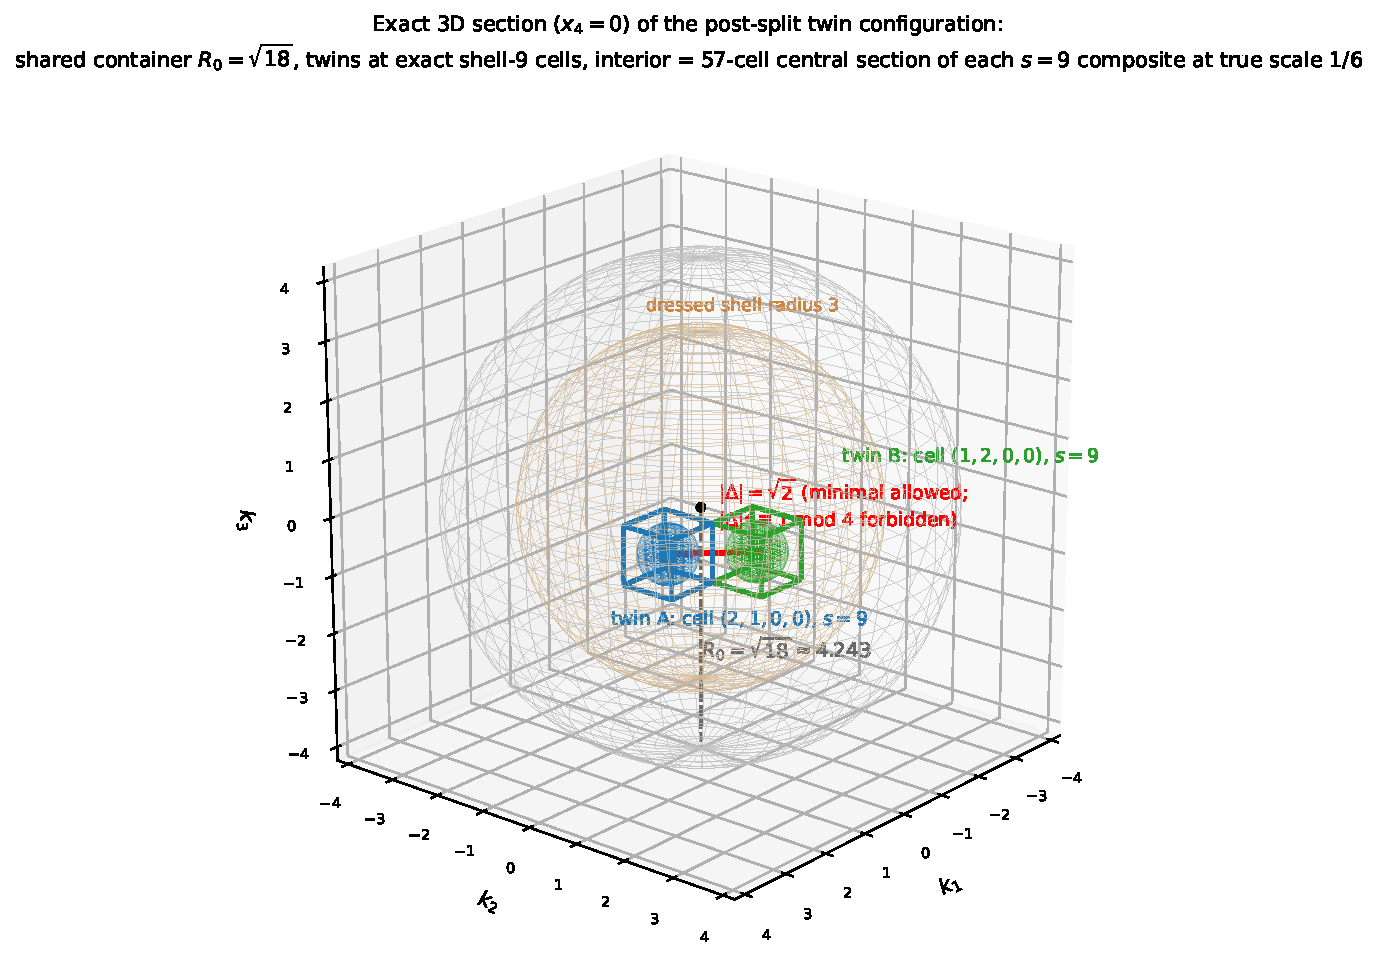
\includegraphics[height=58mm,keepaspectratio]{figure_paper12_2_twin_configuration.pdf}
\end{center}
{\footnotesize 分裂後の双子配置の\textbf{厳密な3次元断面}（$x_4=0$）。共有容器 $R_0=\sqrt{18}$ の中で双子は実在の shell-9 セルを占有し、最小許容分離は $|\Delta|=\sqrt2$（$|\Delta|^2\equiv1$ mod 4 は禁止）。各セル内部は一階層下の137セル複合体の中心断面（57立方体、縮尺 $1/6$）——位置・間隔・縮尺すべて計算値。}
\end{minipage}\hfill
\begin{minipage}[t]{0.30\textwidth}
\secrule{定理の連鎖（論文5$\to$12）}
{\footnotesize
\textbf{5\ 辞書定理}：数え上げ＝零点つき実定在波計数（厳密一致）。$R^2$ は奇数整数に量子化、137/105 問題解消\\[2pt]
\textbf{6\ 凍結定理}：非対称1ビット＝時間様構造の存在条件。記録定理・ヌル構造・不変面積\\[2pt]
\textbf{7\ 排他統計の導出}：安定種 $\{1,3,5\}$・敷居 $s=7$・一意分岐比 $77.4\%:22.6\%$\\[2pt]
\textbf{8\ 会計の反転}：共有曲率$\to$凝縮、内部膨張 $a\propto t^{1/2}$、真空＝面積の貯水池\\[2pt]
\textbf{9\ 半波長検閲}：シフト$\le\frac12$（限界ちょうど）が複合体を保護。存在上限と階層化の強制\\[2pt]
\textbf{10\ 創発ゲージ}：接続の運動学的一意性、ホロノミー $\pi/2$＝測地面積、SO(4) の強制\\[2pt]
\textbf{11\ 次元}：$d=4$ が検閲天井・mod 8・自己双対種子に挟み撃ちで選ばれる\\[2pt]
\textbf{12\ 双子モデル}：測定＝追記（無$\to$有）、もつれのレイヤ解消、隠れ二軸 $R$/$Q$
}
\end{minipage}

\vspace{3pt}
\begin{minipage}[t]{0.64\textwidth}
\begin{center}
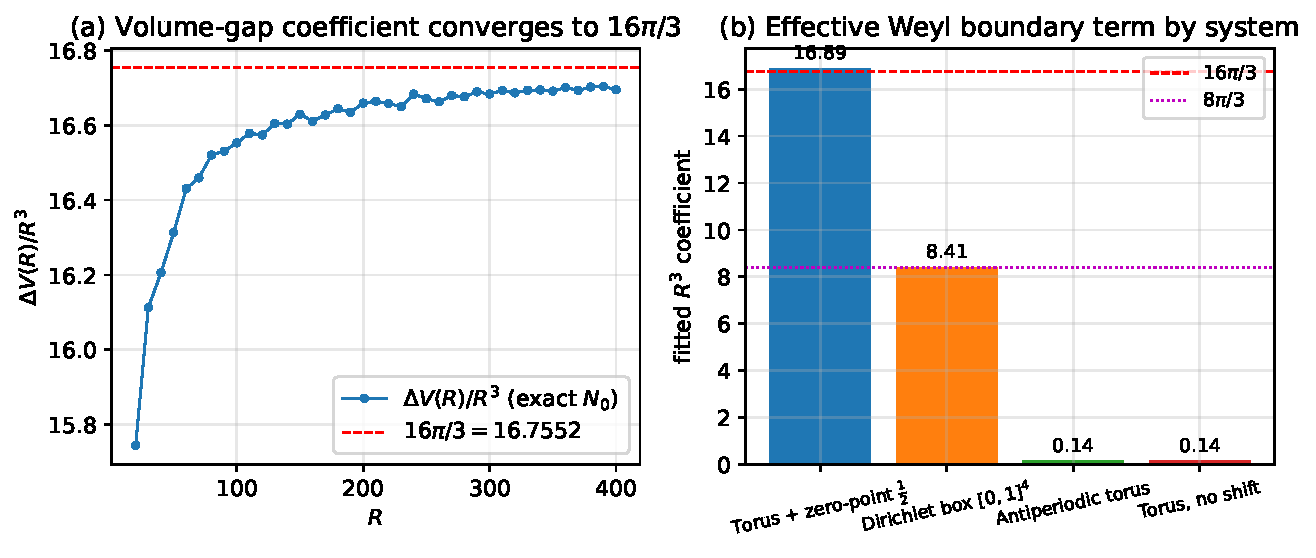
\includegraphics[height=36mm,keepaspectratio]{figure_paper5_1_weyl_gap_convergence.pdf}
\end{center}
\vspace{-4pt}
{\footnotesize \textbf{辞書定理の検証（論文5）}：体積ギャップ係数は $16\pi/3$ に収束（左、厳密 $N_0$、$R\le400$）。右：4境界系の比較——零点シフトは Dirichlet 単位箱の\textbf{ちょうど2倍}の有効 Weyl 境界を生む。}
\end{minipage}\hfill
\begin{minipage}[t]{0.33\textwidth}
\vspace{2pt}
\colorbox{accl}{\begin{minipage}{0.97\linewidth}\vspace{2pt}{\small
\textbf{数列の核}\quad $N_0(R)=1,\ 9,\ 137,\ 473,\ 1545,\ \ldots$\\
条件：$\sum_{i=1}^4(|k_i|+\tfrac12)^2\le R^2$\\[2pt]
零点 $\tfrac12$ $\to$ セル＝実定在波 $\to$ 非重複＝直交 $\to$ 奇数則整合 $\to$ 例外なし分裂 $\to$ $R^2$ の量子化——追加仮定なしの連鎖。}\vspace{2pt}\end{minipage}}
\end{minipage}

\newpage
% ===================== PAGE 2 =====================
\begin{minipage}[t]{0.64\textwidth}
\secrule{展開篇：論文5--12（v0.2、2026-06-11 一斉公開）}
{\small
\begin{tabular}{@{}p{0.30\linewidth}p{0.43\linewidth}p{0.22\linewidth}@{}}
\textbf{5}\ セル＝定在波辞書と半径の量子化 & 辞書定理・零点量子・$16\pi/3$＝Weyl 不足量・分類定理 & \doi{10.5281/zenodo.20640454}\\[2pt]
\textbf{6}\ 保存則・記録・時間様構造 & 凍結定理・$B_4$ ゲージ・$1{+}3$ 極分解・記録定理 & \doi{10.5281/zenodo.20640456}\\[2pt]
\textbf{7}\ 配置統計と関係的読み出し & 排他統計・安定種・分岐比・ホログラフィック読み出し & \doi{10.5281/zenodo.20640458}\\[2pt]
\textbf{8}\ 二つの会計 & 凝縮の最適性・Jeans 型閾値・$a\propto t^{1/2}$・面積法則 & \doi{10.5281/zenodo.20640460}\\[2pt]
\textbf{9}\ 論理波と半波長検閲 & 振幅なし＝整合条件・運動学的安定化・三帯構造 & \doi{10.5281/zenodo.20640462}\\[2pt]
\textbf{10}\ 創発ゲージ構造 & ホロノミー $\pi/2$・SO(4) 強制・スピン持ち上げ・$\beta=0$ & \doi{10.5281/zenodo.20640464}\\[2pt]
\textbf{11}\ 次元の必然性 & 両端点定理 $[0,4]$・mod 8・四脚定理・自己双対種子 & \doi{10.5281/zenodo.20640466}\\[2pt]
\textbf{12}\ 双子最小空間モデル & 測定＝追記・測度分岐・無信号性・仮想変位の認可 & \doi{10.5281/zenodo.20640468}\\
\end{tabular}}
\end{minipage}\hfill
\begin{minipage}[t]{0.33\textwidth}
\secrule{ハイライト}
{\small
\textbf{二階建ての一致}：安定種 $\{1,3,5\}$ と敷居 $s=7$ は、数え上げの階（論文7）と波の階（論文9）という\textbf{独立な計算}で同じ値に到達\\[2pt]
\textbf{公準の削減}：排他原理・測定の収縮・時間の矢・整数格子が、仮定から定理・分解能構造へ\\[2pt]
\textbf{反証可能性}：振幅は曲率と結合できない（論文9）——BMV 型重力媒介もつれ実験が生きた判定者\\[2pt]
\textbf{再導出しないことは欠陥ではない}：移送原理（論文12）。標準理論が公準で済ませた問い（収縮・切断・時間・次元）への解答候補こそが差分}
\end{minipage}

\vspace{6pt}
\begin{minipage}[t]{0.40\textwidth}
\begin{center}
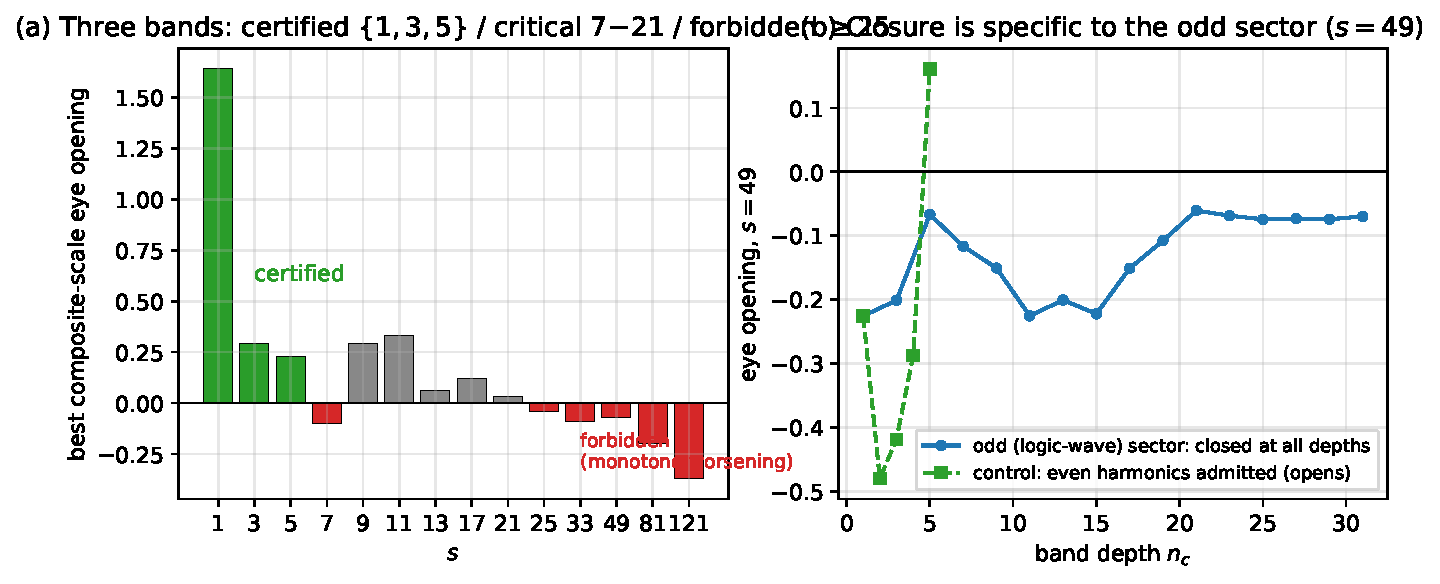
\includegraphics[height=42mm,keepaspectratio]{figure_paper9_3_three_bands.pdf}
\end{center}
\vspace{-4pt}
{\small \textbf{存在の三帯構造（論文9）}：自己証明の余裕は確証帯 $\{1,3,5\}$／臨界帯／禁止帯（$s\ge25$）に分かれ、$s\ge49$ では奇数セクター全帯域で閉鎖（右）。偶数倍音を許せば開く——閉鎖は論理波構造に固有。}
\end{minipage}\hfill
\begin{minipage}[t]{0.29\textwidth}
\begin{center}
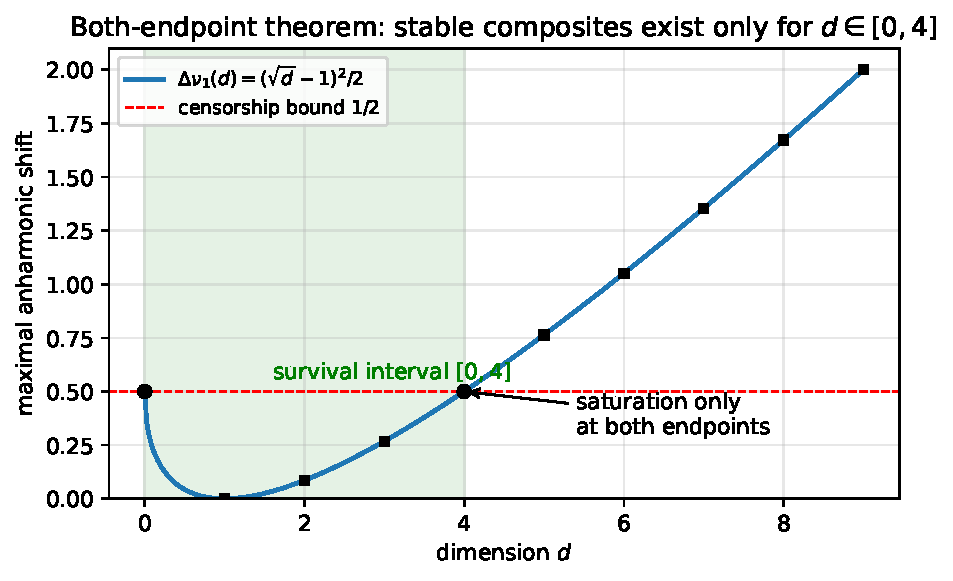
\includegraphics[height=42mm,keepaspectratio]{figure_paper11_1_survival_interval.pdf}
\end{center}
\vspace{-4pt}
{\small \textbf{両端点定理（論文11）}：$\Delta\nu_1(d)=(\sqrt d-1)^2/2\le\frac12 \iff d\in[0,4]$。飽和は両端のみ——$d=4$ は天井で臨界。}
\end{minipage}\hfill
\begin{minipage}[t]{0.27\textwidth}
\begin{center}
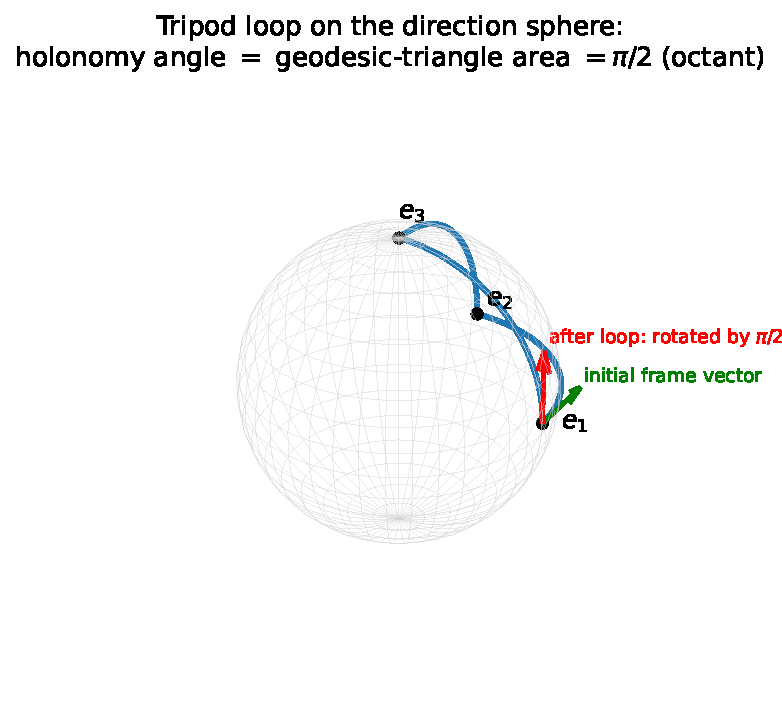
\includegraphics[height=50mm,keepaspectratio]{figure_paper10_1_tripod_holonomy.pdf}
\end{center}
\vspace{-4pt}
{\small \textbf{最初のホロノミー（論文10）}：三脚ループの輸送は $\pi/2$ 回転＝測地三角形（八分円）の面積。離散輸送が連続曲率を厳密に再現。}
\end{minipage}

\vspace{5pt}
{\color{acc}\rule{\textwidth}{1.2pt}}\\[2pt]
{\small \textbf{研究ノート（補遺1--41）・全検証スクリプト・図の生成コード}：\texttt{github.com/WurabeSeiji/ai-chat-logs-open}（「波長空間と周波数空間の双対幾何」フォルダ）\quad
全図は厳密計算（模式図なし）。本シリーズは観察モデルであり、物理理論の導出・修正を主張するものではない。}

\end{document}
